\documentclass[a4paper,12pt]{article}
 \usepackage[utf8]{inputenc}
 \usepackage[left=2cm,top=1cm,right=2cm,bottom=1.5cm,nohead]{geometry}
%\usepackage{wrapfig} % Обтекание рисунков текстом
%\usepackage{floatflt}% Обтекание таблиц текстом
 \usepackage{amsmath} % Математические окружения AMS
 \usepackage{amsfonts} % Шрифты AMS
 \usepackage{amssymb} % Символы AMS
 \usepackage{listings}% to add computer code
 \usepackage{color}
 \definecolor{mygreen}{RGB}{28,172,0} % color values Red, Green, Blue
\definecolor{mylilas}{RGB}{170,55,241}
    \usepackage{graphicx} % Вставить pdf- или png-файлы
  \usepackage{euscript} % Красивый шрифт
%\usepackage{extsizes} % Возможность сделать 14-й шрифт
 \linespread{1.5} % Интерлиньяж
% \usepackage[usenames,dvipsnames,svgnames,table,rgb]{xcolor}% чтоб были гиперссылки и чтоб были цвета

\usepackage{hyperref} % Гиперссылки

%\hypersetup{
% colorlinks = true,
 %linkcolor = MidnightBlue, % ссылки на всякие разделы (их цвет)
 %urlcolor = [rgb]{0,0,1}, % чтоб задавать цыета пиксела - red green blue. не рекомендуется, если потом печатать.
 %citecolor = black
%}
%\usepackage{pdflscape}
%\oddsidemargin=10mm
%\topmargin=-15mm
\usepackage{multicol}
%\hoffset=5mm % см при печати
%\voffset=4.2mm
%\textheight = 720pt
%\textwidth=442pt

\begin{document}
\maketitle \hrulefill
\lstset{language=Matlab,%
    %basicstyle=\color{red},
    breaklines=true,%
    morekeywords={matlab2tikz},
    keywordstyle=\color{blue},%
    morekeywords=[2]{1}, keywordstyle=[2]{\color{black}},
    identifierstyle=\color{black},%
    stringstyle=\color{mylilas},
    commentstyle=\color{mygreen},%
    showstringspaces=false,%without this there will be a symbol in the places where there is a space
    numbers=left,%
    numberstyle={\tiny \color{black}},% size of the numbers
    numbersep=9pt, % this defines how far the numbers are from the text
    emph=[1]{for,end,break},emphstyle=[1]\color{red}, %some words to emphasise
    %emph=[2]{word1,word2}, emphstyle=[2]{style},
}

\begin{center}

\textbf {\Large{Empirircal Methods HA 1}}\\
Konstantin Guryev\\
Pennsylvania State University\\
2018
\end{center}

\textbf{Problem \textnumero \,1 }
See the pic1.


\begin{figure}[h]
\centering
%\begin{center}
\includegraphics[width=16cm,height=8cm,keepaspectratio]{Figure1.eps}
%\caption{Движущийся жесткий штамп}
%\caption{pic1}
%\end{center}
\end{figure}

\textbf{Problem \textnumero \,2 }
The sum is equal to $1000$
\vspace{\baselineskip}

\textbf{Problem \textnumero \,3 }
\vspace{\baselineskip}

C =
\begin{pmatrix}
  29 \\
  133\\
  43
\end{pmatrix};
D = 
\begin{pmatrix}
  -3.2505 \\
  0.3961 \\
  0.8037
\end{pmatrix};
E = $205$;
F = 
\begin{pmatrix}
  2& 4\\
  3& 12
\end{pmatrix};
x = 
\begin{pmatrix}
  -0.1622 \\
  1.2432 \\
  -1.1081
\end{pmatrix}.
\vspace{\baselineskip}

\textbf{Problem \textnumero \,4 }
One liner code. I think there is no need in attaching the resulting matrix.
\vspace{\baselineskip}

\textbf{Problem \textnumero \,5 }
\vspace{\baselineskip}

$L$ = 
\begin{pmatrix}
  8.0642& 6.7597& 10.4107 \\
  9.6053& 10.7458& 8.9353 \\
  11.7697& 10.8751& 11.9275 \\
  7.0215& 11.0100& 6.9552 \\
  4.7903& 9.7087& 11.0175 
\end{pmatrix};
$L_{new}$ = 
\begin{pmatrix}
  0& 0& 1 \\
  0& 1& 0 \\
  1& 1& 1 \\
  0& 1& 0 \\
  0& 0& 1 
\end{pmatrix}.
\vspace{\baselineskip}

\textbf{Problem \textnumero \,6 }
\vspace{\baselineskip}

\[\hat{\beta}=\begin{bmatrix}
0.0817\\
0.1201\\
0.1399\\
0.0295
\end{bmatrix};
\hat{\sigma}_{\beta}=\begin{bmatrix}
0.0193\\
0.0061\\
0.0089\\
0.0020
\end{bmatrix}\]


\newpage
\section*{Matlab Code} \lstinputlisting{HA_1.m}

\end{document}